\documentclass{article}

\usepackage{arxiv}

\usepackage[utf8]{inputenc} % allow utf-8 input
\usepackage[T1]{fontenc}    % use 8-bit T1 fonts
\usepackage{lmodern}        % https://github.com/rstudio/rticles/issues/343
\usepackage{hyperref}       % hyperlinks
\usepackage{url}            % simple URL typesetting
\usepackage{booktabs}       % professional-quality tables
\usepackage{amsfonts}       % blackboard math symbols
\usepackage{nicefrac}       % compact symbols for 1/2, etc.
\usepackage{microtype}      % microtypography
\usepackage{lipsum}
\usepackage{graphicx}

\title{ggsignif: R Package for Displaying Significance Brackets for
`ggplot2'}

\author{
    Constantin Ahlmann-Eltze
   \\
    The European Molecular Biology Laboratory, Heidelberg, Germany \\
   \\
  \texttt{} \\
   \And
    Indrajeet Patil
   \\
    Center for Humans and Machines, Max Planck Institute for Human
Development, Berlin, Germany \\
   \\
  \texttt{} \\
  }

\usepackage{color}
\usepackage{fancyvrb}
\newcommand{\VerbBar}{|}
\newcommand{\VERB}{\Verb[commandchars=\\\{\}]}
\DefineVerbatimEnvironment{Highlighting}{Verbatim}{commandchars=\\\{\}}
% Add ',fontsize=\small' for more characters per line
\usepackage{framed}
\definecolor{shadecolor}{RGB}{248,248,248}
\newenvironment{Shaded}{\begin{snugshade}}{\end{snugshade}}
\newcommand{\AlertTok}[1]{\textcolor[rgb]{0.94,0.16,0.16}{#1}}
\newcommand{\AnnotationTok}[1]{\textcolor[rgb]{0.56,0.35,0.01}{\textbf{\textit{#1}}}}
\newcommand{\AttributeTok}[1]{\textcolor[rgb]{0.77,0.63,0.00}{#1}}
\newcommand{\BaseNTok}[1]{\textcolor[rgb]{0.00,0.00,0.81}{#1}}
\newcommand{\BuiltInTok}[1]{#1}
\newcommand{\CharTok}[1]{\textcolor[rgb]{0.31,0.60,0.02}{#1}}
\newcommand{\CommentTok}[1]{\textcolor[rgb]{0.56,0.35,0.01}{\textit{#1}}}
\newcommand{\CommentVarTok}[1]{\textcolor[rgb]{0.56,0.35,0.01}{\textbf{\textit{#1}}}}
\newcommand{\ConstantTok}[1]{\textcolor[rgb]{0.00,0.00,0.00}{#1}}
\newcommand{\ControlFlowTok}[1]{\textcolor[rgb]{0.13,0.29,0.53}{\textbf{#1}}}
\newcommand{\DataTypeTok}[1]{\textcolor[rgb]{0.13,0.29,0.53}{#1}}
\newcommand{\DecValTok}[1]{\textcolor[rgb]{0.00,0.00,0.81}{#1}}
\newcommand{\DocumentationTok}[1]{\textcolor[rgb]{0.56,0.35,0.01}{\textbf{\textit{#1}}}}
\newcommand{\ErrorTok}[1]{\textcolor[rgb]{0.64,0.00,0.00}{\textbf{#1}}}
\newcommand{\ExtensionTok}[1]{#1}
\newcommand{\FloatTok}[1]{\textcolor[rgb]{0.00,0.00,0.81}{#1}}
\newcommand{\FunctionTok}[1]{\textcolor[rgb]{0.00,0.00,0.00}{#1}}
\newcommand{\ImportTok}[1]{#1}
\newcommand{\InformationTok}[1]{\textcolor[rgb]{0.56,0.35,0.01}{\textbf{\textit{#1}}}}
\newcommand{\KeywordTok}[1]{\textcolor[rgb]{0.13,0.29,0.53}{\textbf{#1}}}
\newcommand{\NormalTok}[1]{#1}
\newcommand{\OperatorTok}[1]{\textcolor[rgb]{0.81,0.36,0.00}{\textbf{#1}}}
\newcommand{\OtherTok}[1]{\textcolor[rgb]{0.56,0.35,0.01}{#1}}
\newcommand{\PreprocessorTok}[1]{\textcolor[rgb]{0.56,0.35,0.01}{\textit{#1}}}
\newcommand{\RegionMarkerTok}[1]{#1}
\newcommand{\SpecialCharTok}[1]{\textcolor[rgb]{0.00,0.00,0.00}{#1}}
\newcommand{\SpecialStringTok}[1]{\textcolor[rgb]{0.31,0.60,0.02}{#1}}
\newcommand{\StringTok}[1]{\textcolor[rgb]{0.31,0.60,0.02}{#1}}
\newcommand{\VariableTok}[1]{\textcolor[rgb]{0.00,0.00,0.00}{#1}}
\newcommand{\VerbatimStringTok}[1]{\textcolor[rgb]{0.31,0.60,0.02}{#1}}
\newcommand{\WarningTok}[1]{\textcolor[rgb]{0.56,0.35,0.01}{\textbf{\textit{#1}}}}

% Pandoc citation processing
\newlength{\csllabelwidth}
\setlength{\csllabelwidth}{3em}
\newlength{\cslhangindent}
\setlength{\cslhangindent}{1.5em}
% for Pandoc 2.8 to 2.10.1
\newenvironment{cslreferences}%
  {}%
  {\par}
% For Pandoc 2.11+
\newenvironment{CSLReferences}[3] % #1 hanging-ident, #2 entry spacing
 {% don't indent paragraphs
  \setlength{\parindent}{0pt}
  % turn on hanging indent if param 1 is 1
  \ifodd #1 \everypar{\setlength{\hangindent}{\cslhangindent}}\ignorespaces\fi
  % set entry spacing
  \ifnum #2 > 0
  \setlength{\parskip}{#2\baselineskip}
  \fi
 }%
 {}
\usepackage{calc} % for calculating minipage widths
\newcommand{\CSLBlock}[1]{#1\hfill\break}
\newcommand{\CSLLeftMargin}[1]{\parbox[t]{\csllabelwidth}{#1}}
\newcommand{\CSLRightInline}[1]{\parbox[t]{\linewidth - \csllabelwidth}{#1}}
\newcommand{\CSLIndent}[1]{\hspace{\cslhangindent}#1}



\begin{document}
\maketitle

\def\tightlist{}


\begin{abstract}
Research hypotheses are often concerned with the difference between two
groups and statistical tests provide indicators (like \emph{p}-values or
Bayes factors) about the evidence for or against such differences. The R
package, \texttt{ggsignif} provides a quick way to visualize such
pairwise indicators as an annotation in a plot, for example showing if a
difference is statistically significant. \texttt{ggsignif} follows the
principles of the grammar of graphics
(\protect\hyperlink{ref-Wilkinson2012}{Wilkinson, 2012}) and provides a
new layer that can be added to plots made with the \texttt{ggplot2}
package (\protect\hyperlink{ref-Wickham2016}{Wickham, 2016}).
\end{abstract}

\keywords{
    R
   \and
    ggplot2
   \and
    ggplot2-extension
  }

\hypertarget{statement-of-need}{%
\section{Statement of Need}\label{statement-of-need}}

During the exploratory analysis of data with discrete covariates,
researchers commonly start with a one-way ANOVA to see if there are any
differences in the group means. This is typically followed up with
multiple comparisons to see if specific levels of the discrete
covariates differ significantly. The \texttt{ggsignif} package provides
a way to graphically display all or a few (depending on the context of
the research hypotheses) of such comparisons. It is also used by other R
package developers as the back-end for graphical display of pairwise
comparisons, such as \texttt{ggpubr}
(\protect\hyperlink{ref-Kassambara2020}{Kassambara, 2020}),
\texttt{ggstatsplot} (\protect\hyperlink{ref-Patil2018}{Patil, 2018}),
and more. These packages demonstrate how \texttt{ggsignif} can be
extended to display results from any type of pairwise comparisons test
(e.g., Bayesian \emph{t}-test, Dunn test, etc.).

\hypertarget{features}{%
\section{Features}\label{features}}

The following is a simple example demonstrating how a group difference
can be annotated using \texttt{geom\_signif} layers from
\texttt{ggsignif} package.

\begin{Shaded}
\begin{Highlighting}[]
\FunctionTok{set.seed}\NormalTok{(}\DecValTok{123}\NormalTok{)}
\FunctionTok{library}\NormalTok{(ggplot2)}
\FunctionTok{library}\NormalTok{(ggsignif)}

\FunctionTok{ggplot}\NormalTok{(mpg, }\FunctionTok{aes}\NormalTok{(class, hwy)) }\SpecialCharTok{+}
  \FunctionTok{geom\_boxplot}\NormalTok{() }\SpecialCharTok{+}
  \FunctionTok{geom\_signif}\NormalTok{(}
    \AttributeTok{comparisons =} \FunctionTok{list}\NormalTok{(}\FunctionTok{c}\NormalTok{(}\StringTok{"compact"}\NormalTok{, }\StringTok{"midsize"}\NormalTok{), }\FunctionTok{c}\NormalTok{(}\StringTok{"minivan"}\NormalTok{, }\StringTok{"suv"}\NormalTok{)),}
    \AttributeTok{map\_signif\_level =} \ConstantTok{TRUE}
\NormalTok{  ) }\SpecialCharTok{+}
  \FunctionTok{ylim}\NormalTok{(}\ConstantTok{NA}\NormalTok{, }\DecValTok{48}\NormalTok{)}
\end{Highlighting}
\end{Shaded}

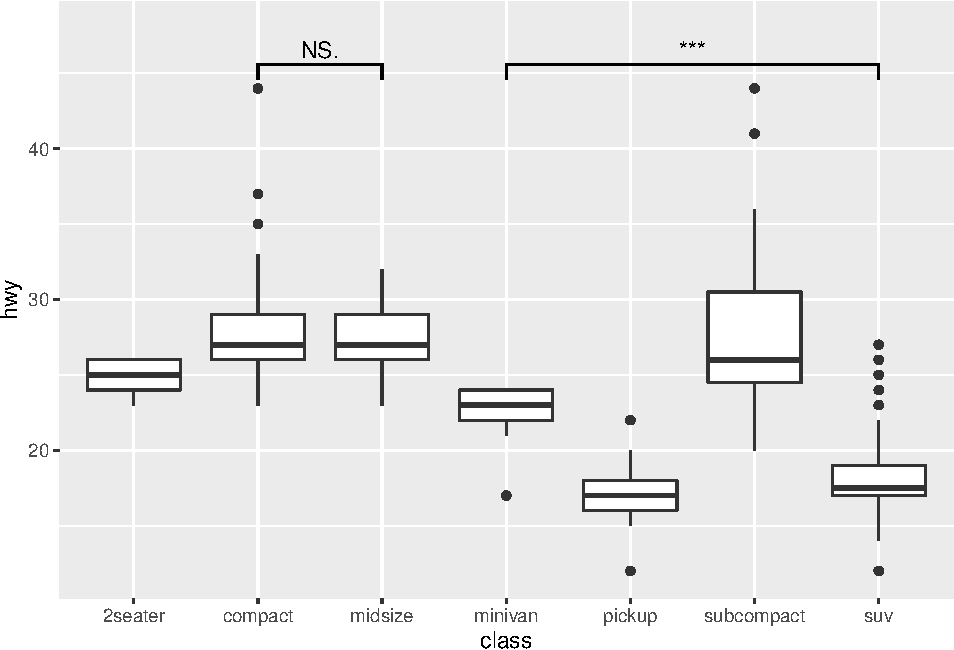
\includegraphics[width=1\linewidth]{paper_files/figure-latex/simpe_comparison-1}

For more advanced examples, the readers are encouraged to read the
package website: \url{https://const-ae.github.io/ggsignif/}.

\hypertarget{licensing-and-availability}{%
\section{Licensing and Availability}\label{licensing-and-availability}}

\texttt{ggsignif} is licensed under the GNU General Public License
(v3.0), with all source code stored at
\href{https://github.com/const-ae/ggsignif}{GitHub}, and with a
corresponding issue tracker for bug reporting and feature enhancements.
In the spirit of honest and open science, we encourage requests/tips for
fixes, feature updates, as well as general questions and concerns via
direct interaction with contributors and developers, by
\href{https://github.com/const-ae/ggsignif/issues}{filing an issue}. See
the
\href{https://github.com/const-ae/ggsignif/blob/master/CODE_OF_CONDUCT.md}{\emph{Contribution
Guidelines}} for this package.

\hypertarget{acknowledgements}{%
\section{Acknowledgements}\label{acknowledgements}}

We would like to thank the users of \texttt{ggsignif} package for
reporting bugs and for providing valuable feedback.

This work was supported by the EMBL International PhD Programme
(C.A.E.).

\hypertarget{references}{%
\section*{References}\label{references}}
\addcontentsline{toc}{section}{References}

\hypertarget{refs}{}
\begin{CSLReferences}{1}{0}
\leavevmode\hypertarget{ref-Kassambara2020}{}%
Kassambara, A. (2020). \emph{{ggpubr}: '{ggplot2}' based publication
ready plots}. Retrieved from
\url{https://CRAN.R-project.org/package=ggpubr}

\leavevmode\hypertarget{ref-Patil2018}{}%
Patil, I. (2018). {ggstatsplot}: '{ggplot2}' based plots with
statistical details. \emph{CRAN}.
doi:\href{https://doi.org/10.5281/zenodo.2074621}{10.5281/zenodo.2074621}

\leavevmode\hypertarget{ref-Wickham2016}{}%
Wickham, H. (2016). \emph{{ggplot2}: Elegant graphics for data
analysis}. Springer-Verlag New York. Retrieved from
\url{https://ggplot2.tidyverse.org}

\leavevmode\hypertarget{ref-Wilkinson2012}{}%
Wilkinson, L. (2012). The grammar of graphics. \emph{Handbook of
computational statistics} (pp. 375--414). Springer.

\end{CSLReferences}

\bibliographystyle{unsrt}
\bibliography{paper.bib}


\end{document}
